\hypertarget{group__core__template}{}\section{Template types}
\label{group__core__template}\index{Template types@{Template types}}


The generic template types used as the basis for the core types.  


Collaboration diagram for Template types\+:\nopagebreak
\begin{figure}[H]
\begin{center}
\leavevmode
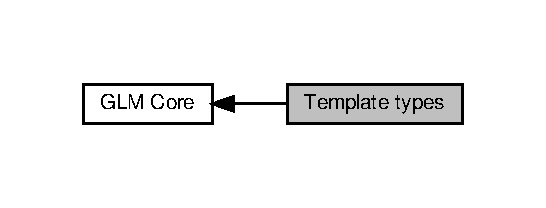
\includegraphics[width=262pt]{group__core__template}
\end{center}
\end{figure}
The generic template types used as the basis for the core types. 

These types are all templates used to define the actual \hyperlink{group__core__types}{Types}. These templetes are implementation details of G\+LM types and should not be used explicitly. 